% ============================================================================
% Workshop variant of the OLMo-2-7B RLHF case study.
% Differences from sections/07_6_rlhf.tex:
%   - Promoted from \subsection to \section (no §7 Experiments parent in
%     the workshop wrapper).
%   - One-paragraph framing intro added so this section is read as the
%     AI-side anchor (parallel to Tevet as the Human-side anchor).
%   - Cross-model comparison trimmed to a one-sentence pointer to the
%     appendix; full table and discussion live in sections/07_6_rlhf.tex
%     which is appendix-only in the workshop wrapper.
%   - Released-artifacts URL replaced with anonymous-mirror placeholder
%     for double-blind review (Phase 4 finalizes the workaround).
% ============================================================================

% Load generated macros BEFORE the section body so prose references resolve.
\IfFileExists{../results/rlhf_experiment/paper_macros_rlhf.tex}{%
  % Auto-generated by scripts/rlhf_experiment/5_analyze_and_figures.py

\newcommand{\olmoAlpacaBaseDMean}{0.488}
\newcommand{\olmoAlpacaSftDMean}{0.330}
\newcommand{\olmoAlpacaDpoDMean}{0.290}
\newcommand{\olmoAlpacaInstructDMean}{0.285}
\newcommand{\olmoAlpacaHoneAPbonf}{0.000}
\newcommand{\olmoAlpacaHoneADz}{1.614}
\newcommand{\olmoAlpacaHoneADiff}{0.158}
\newcommand{\olmoAlpacaHoneBPbonf}{0.000}
\newcommand{\olmoAlpacaHoneBDz}{0.577}
\newcommand{\olmoAlpacaHoneBDiff}{0.040}
\newcommand{\olmoAlpacaHoneCPbonf}{0.000}
\newcommand{\olmoAlpacaHoneCDz}{2.526}
\newcommand{\olmoAlpacaHoneCDiff}{0.202}
\newcommand{\olmoAlpacaHpaP}{0.000}
\newcommand{\olmoAlpacaHpaDz}{0.222}
\newcommand{\olmoAlpacaHpaDiff}{0.005}
\newcommand{\olmoAlpacaN}{200}
\newcommand{\olmoNbCuratedBaseDMean}{0.498}
\newcommand{\olmoNbCuratedSftDMean}{0.384}
\newcommand{\olmoNbCuratedDpoDMean}{0.318}
\newcommand{\olmoNbCuratedInstructDMean}{0.315}
\newcommand{\olmoNbCuratedHoneAPbonf}{0.000}
\newcommand{\olmoNbCuratedHoneADz}{1.232}
\newcommand{\olmoNbCuratedHoneADiff}{0.113}
\newcommand{\olmoNbCuratedHoneBPbonf}{0.000}
\newcommand{\olmoNbCuratedHoneBDz}{0.897}
\newcommand{\olmoNbCuratedHoneBDiff}{0.066}
\newcommand{\olmoNbCuratedHoneCPbonf}{0.000}
\newcommand{\olmoNbCuratedHoneCDz}{2.054}
\newcommand{\olmoNbCuratedHoneCDiff}{0.183}
\newcommand{\olmoNbCuratedHpaP}{0.016}
\newcommand{\olmoNbCuratedHpaDz}{0.069}
\newcommand{\olmoNbCuratedHpaDiff}{0.004}
\newcommand{\olmoNbCuratedN}{100}
%
}{}
\IfFileExists{../results/rlhf_experiment/paper_macros_rlhf_lenmatched.tex}{%
  % Auto-generated by scripts/rlhf_experiment/5_analyze_and_figures.py

\newcommand{\olmoLmAlpacaBaseDMean}{0.481}
\newcommand{\olmoLmAlpacaSftDMean}{0.329}
\newcommand{\olmoLmAlpacaDpoDMean}{0.286}
\newcommand{\olmoLmAlpacaInstructDMean}{0.281}
\newcommand{\olmoLmAlpacaHoneAPbonf}{0.000}
\newcommand{\olmoLmAlpacaHoneADz}{1.615}
\newcommand{\olmoLmAlpacaHoneADiff}{0.151}
\newcommand{\olmoLmAlpacaHoneBPbonf}{0.000}
\newcommand{\olmoLmAlpacaHoneBDz}{0.675}
\newcommand{\olmoLmAlpacaHoneBDiff}{0.044}
\newcommand{\olmoLmAlpacaHoneCPbonf}{0.000}
\newcommand{\olmoLmAlpacaHoneCDz}{2.425}
\newcommand{\olmoLmAlpacaHoneCDiff}{0.200}
\newcommand{\olmoLmAlpacaHpaP}{0.004}
\newcommand{\olmoLmAlpacaHpaDz}{0.227}
\newcommand{\olmoLmAlpacaHpaDiff}{0.005}
\newcommand{\olmoLmAlpacaN}{150}
\newcommand{\olmoLmNbCuratedBaseDMean}{0.481}
\newcommand{\olmoLmNbCuratedSftDMean}{0.369}
\newcommand{\olmoLmNbCuratedDpoDMean}{0.312}
\newcommand{\olmoLmNbCuratedInstructDMean}{0.303}
\newcommand{\olmoLmNbCuratedHoneAPbonf}{0.000}
\newcommand{\olmoLmNbCuratedHoneADz}{1.212}
\newcommand{\olmoLmNbCuratedHoneADiff}{0.112}
\newcommand{\olmoLmNbCuratedHoneBPbonf}{0.000}
\newcommand{\olmoLmNbCuratedHoneBDz}{0.957}
\newcommand{\olmoLmNbCuratedHoneBDiff}{0.057}
\newcommand{\olmoLmNbCuratedHoneCPbonf}{0.000}
\newcommand{\olmoLmNbCuratedHoneCDz}{1.889}
\newcommand{\olmoLmNbCuratedHoneCDiff}{0.179}
\newcommand{\olmoLmNbCuratedHpaP}{0.028}
\newcommand{\olmoLmNbCuratedHpaDz}{0.375}
\newcommand{\olmoLmNbCuratedHpaDiff}{0.010}
\newcommand{\olmoLmNbCuratedN}{39}
%
}{}
\IfFileExists{../results/rlhf_experiment/tables/cross_model_macros.tex}{%
  % Auto-generated by scripts/rlhf_experiment/5c_cross_model_table.py

\newcommand{\crossModelQwenFourB}{0.241}
\newcommand{\crossModelQwenEightB}{0.210}
\newcommand{\crossModelQwenTwoThreeFiveB}{0.209}
\newcommand{\crossModelLlamaThreeThreeSeventyB}{0.169}
\newcommand{\crossModelGptFiveNano}{0.260}
\newcommand{\crossModelGptFive}{0.262}
\newcommand{\crossModelClaudeSonnetFourFive}{0.171}
\newcommand{\crossModelOlmoBase}{0.485}
\newcommand{\crossModelOlmoSft}{0.330}
\newcommand{\crossModelOlmoDpo}{0.299}
\newcommand{\crossModelOlmoInstruct}{0.283}
%
}{}

\section{OLMo-2-7B Post-Training: AI-Side Validation}\label{sec:rlhf-experiment}

The Tevet evaluation in Section~\ref{sec:tevet} validates $D_{Ca_n}$ against human-grounded labels.
This section closes the loop on the AI side: sample from real policies at four post-training stages of the same base model and ask whether $D_{Ca_n}$ detects the diversity loss widely attributed to RLHF \citep{kirk2023rlhf,zhang2025verbalizedsampling,padmakumar2023writingreduces}.
Because the same pipeline scores both human-written and AI-generated response sets, this and the previous section read as two halves of the same evaluation: the metric is policy-agnostic, and the evidence we present matches both halves of the workshop's ``Human-AI'' framing.

\paragraph{Setup.} We sample from the four released stages of the OLMo-2-1124-7B pipeline \citep{olmo2024olmo2}: the pretrained base model, its SFT checkpoint, the DPO checkpoint trained on preference data, and the final RLVR-tuned Instruct checkpoint.
On two prompt sets, \olmoAlpacaN{} AlpacaEval prompts \citep{dubois2024alpacafarm} (seed=42 subsample of 805) and \olmoNbCuratedN{} curated NoveltyBench prompts \citep{zhang2025noveltybench}, we draw $K{=}10$ responses per prompt per stage (temperature 1.0, top-$p$ 1.0, $\texttt{max\_new\_tokens}{=}100$).
Base runs raw; SFT / DPO / Instruct receive the prompt through their own chat template.
We score each (stage, prompt) group with $D_{Ca_n}$ using Qwen2.5-3B as $\theta$ and 25 permutations.
For comparison we also compute Kirk et al.'s EAD and distinct-$n$ (averaged over $n{=}1\ldots5$) and SentBERT similarity-to-diversity \citep{reimers2019sbert}.

\paragraph{Hypotheses.} We pre-register three one-sided paired Wilcoxon signed-rank tests \citep{dror2018hitchhiker} with family-wise Bonferroni correction across the three contrasts \citep{dror2017replicability} ($\alpha = 0.05/3$):

\begin{itemize}[nosep]
    \item \textbf{H1a} $D_{\mathrm{base}} > D_{\mathrm{SFT}}$: SFT narrows toward the helpful-assistant style.
    \item \textbf{H1b} $D_{\mathrm{SFT}} > D_{\mathrm{DPO}}$: DPO is trained on preference data and inherits its typicality bias \citep{zhang2025verbalizedsampling}.
    \item \textbf{H1c} $D_{\mathrm{base}} > D_{\mathrm{RLVR}}$: cumulative effect of the full post-training pipeline.
\end{itemize}

The DPO-vs-RLVR comparison is reported as an exploratory two-sided contrast (H1$'$): RLVR uses \emph{verifiable} rewards (math and instruction-following \citep{olmo2024olmo2}) rather than human preferences, so the typicality-bias mechanism that motivates H1b does not obviously apply to it.

\paragraph{Results.}

\begin{table}[h]
\centering
\caption{Per-prompt $D_{Ca_n}$ by OLMo-2-7B stage, with pre-registered paired tests.}
\label{tab:rlhf-diversity}
\small
\IfFileExists{../results/rlhf_experiment/tables/rlhf_diversity.tex}{%
  \begin{tabular}{lrrr}
\toprule
Stage & $D = C \cdot a_n$ mean & std & $n$ \\
\midrule
Base & 0.488 & 0.045 & 200 \\
SFT & 0.330 & 0.093 & 200 \\
DPO & 0.290 & 0.068 & 200 \\
Instruct (RLVR) & 0.285 & 0.071 & 200 \\
\midrule
\multicolumn{4}{l}{\textbf{H1 tests (paired Wilcoxon, Bonferroni)}} \\
Base$>$ SFT & $\Delta=0.158$ & $d_z=1.614$ & $p=<0.001$ \\
SFT$>$ DPO & $\Delta=0.040$ & $d_z=0.577$ & $p=<0.001$ \\
Base$>$ Instruct (RLVR) & $\Delta=0.202$ & $d_z=2.526$ & $p=<0.001$ \\
\multicolumn{4}{l}{\textbf{H1' (exploratory two-sided, uncorrected)}} \\
DPO $\neq$ Instruct & $\Delta=0.005$ & $d_z=0.222$ & $p=<0.001$ \\
\bottomrule
\end{tabular}

\vspace{0.5em}

\begin{tabular}{lrrr}
\toprule
Stage & $D = C \cdot a_n$ mean & std & $n$ \\
\midrule
Base & 0.498 & 0.030 & 100 \\
SFT & 0.384 & 0.089 & 100 \\
DPO & 0.318 & 0.073 & 100 \\
Instruct (RLVR) & 0.315 & 0.086 & 100 \\
\midrule
\multicolumn{4}{l}{\textbf{H1 tests (paired Wilcoxon, Bonferroni)}} \\
Base$>$ SFT & $\Delta=0.113$ & $d_z=1.232$ & $p=<0.001$ \\
SFT$>$ DPO & $\Delta=0.066$ & $d_z=0.897$ & $p=<0.001$ \\
Base$>$ Instruct (RLVR) & $\Delta=0.183$ & $d_z=2.054$ & $p=<0.001$ \\
\multicolumn{4}{l}{\textbf{H1' (exploratory two-sided, uncorrected)}} \\
DPO $\neq$ Instruct & $\Delta=0.004$ & $d_z=0.069$ & $p=0.016$ \\
\bottomrule
\end{tabular}

\vspace{0.5em}
%
}{%
  \texttt{[table will appear here after \texttt{5\_analyze\_and\_figures.py} runs]}%
}
\end{table}

Table~\ref{tab:rlhf-diversity} reports per-stage means, the pre-registered contrasts, and the exploratory DPO$\,\neq\,$RLVR test.
On AlpacaEval, $D_{Ca_n}$ drops from \olmoAlpacaBaseDMean{} (base) to \olmoAlpacaSftDMean{} (SFT) to \olmoAlpacaDpoDMean{} (DPO) to \olmoAlpacaInstructDMean{} (Instruct/RLVR).
All three pre-registered contrasts are significant after Bonferroni correction: H1a (base$\,\rightarrow\,$SFT) has $d_z = \olmoAlpacaHoneADz$, $p_\mathrm{Bonf} = \olmoAlpacaHoneAPbonf$; H1b (SFT$\,\rightarrow\,$DPO) has $d_z = \olmoAlpacaHoneBDz$, $p_\mathrm{Bonf} = \olmoAlpacaHoneBPbonf$; H1c (base$\,\rightarrow\,$RLVR) has $d_z = \olmoAlpacaHoneCDz$, $p_\mathrm{Bonf} = \olmoAlpacaHoneCPbonf$.
On NoveltyBench curated the corresponding means are \olmoNbCuratedBaseDMean / \olmoNbCuratedSftDMean / \olmoNbCuratedDpoDMean / \olmoNbCuratedInstructDMean, with H1a $d_z = \olmoNbCuratedHoneADz$ ($p_\mathrm{Bonf} = \olmoNbCuratedHoneAPbonf$), H1b $d_z = \olmoNbCuratedHoneBDz$ ($p_\mathrm{Bonf} = \olmoNbCuratedHoneBPbonf$), and H1c $d_z = \olmoNbCuratedHoneCDz$ ($p_\mathrm{Bonf} = \olmoNbCuratedHoneCPbonf$).
Figure~\ref{fig:rlhf-ak-violin} shows the underlying $\bar{a}_k$ curves and per-prompt $D_{Ca_n}$ distributions: each later stage's curve lies below the base curve at every $k \geq 2$, and the per-prompt distribution shifts toward lower $D_{Ca_n}$ as the pipeline advances.

\IfFileExists{../figures/rlhf_experiment/ak_curves_overlay_alpacaeval.pdf}{%
\begin{figure*}[h]
\centering
\begin{subfigure}[t]{0.48\textwidth}
    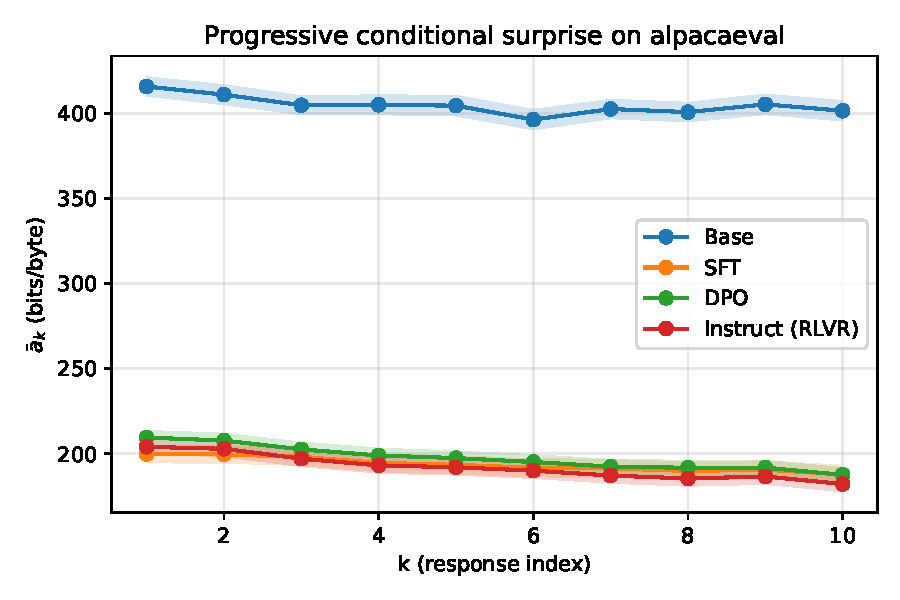
\includegraphics[width=\textwidth]{../figures/rlhf_experiment/ak_curves_overlay_alpacaeval.pdf}
    \caption{AlpacaEval $\bar{a}_k$ curves.}
\end{subfigure}\hfill
\begin{subfigure}[t]{0.48\textwidth}
    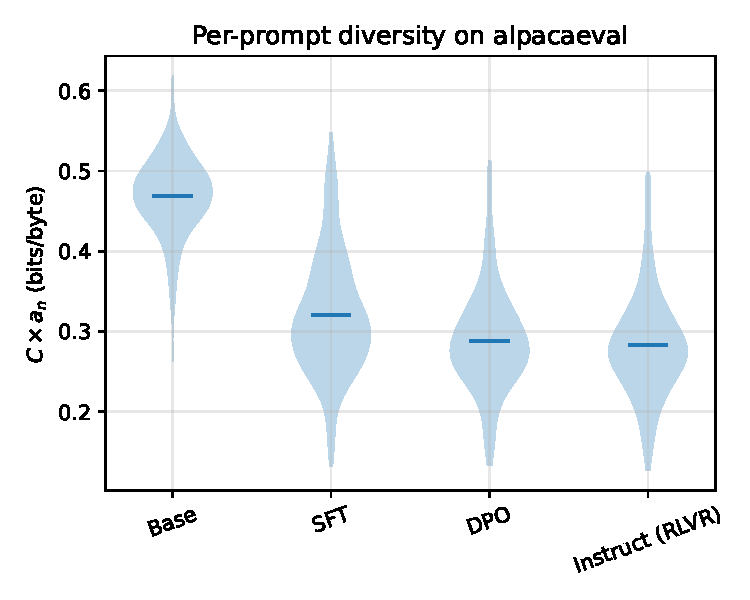
\includegraphics[width=\textwidth]{../figures/rlhf_experiment/per_prompt_D_violin_alpacaeval.pdf}
    \caption{Per-prompt $D_{Ca_n}$ by stage.}
\end{subfigure}
\caption{Progressive conditional surprise curves and per-prompt diversity distributions across the four OLMo-2-7B stages on AlpacaEval. Each later stage's $\bar{a}_k$ curve lies below the base curve at every $k \geq 2$; the per-prompt $D_{Ca_n}$ distribution shifts toward lower values as the pipeline advances.}
\label{fig:rlhf-ak-violin}
\end{figure*}
}{}

\IfFileExists{../figures/rlhf_experiment/metric_correlation_scatter_alpacaeval_lm.pdf}{%
\begin{figure*}[!htbp]
\centering
\begin{subfigure}[t]{\textwidth}
    \centering
    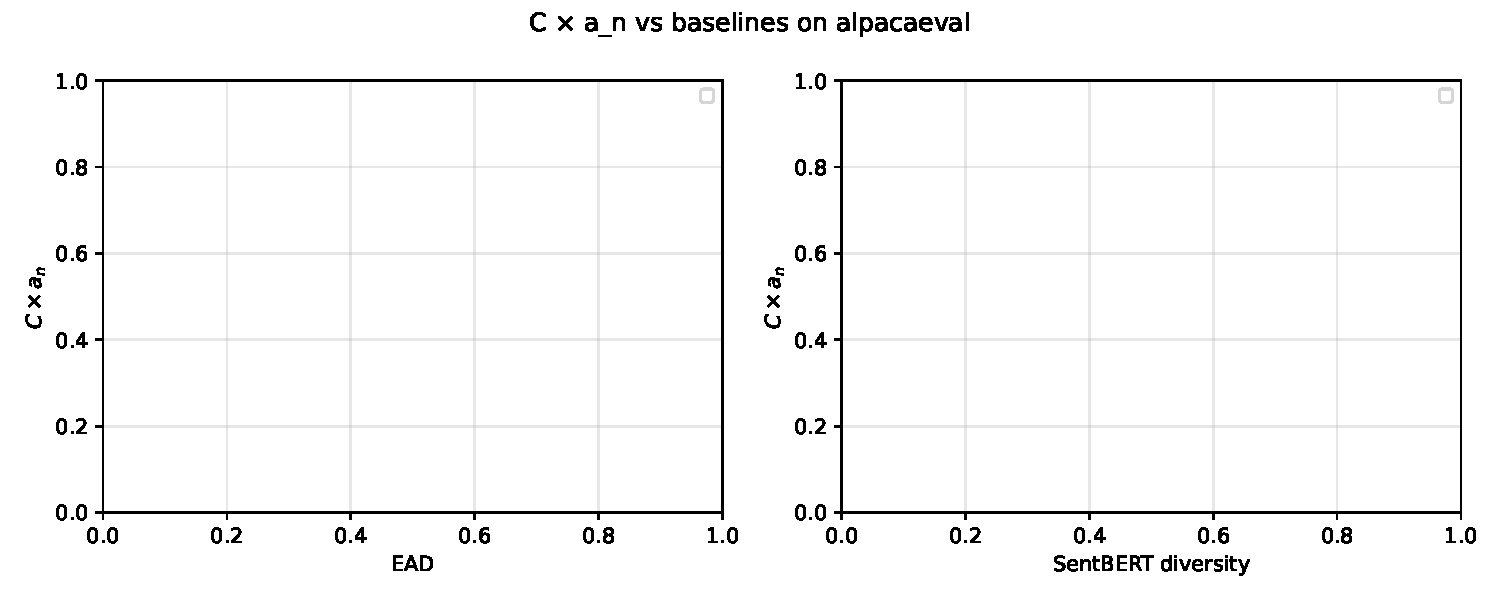
\includegraphics[width=0.85\textwidth]{../figures/rlhf_experiment/metric_correlation_scatter_alpacaeval_lm.pdf}
    \caption{AlpacaEval (length-matched, $n=\olmoLmAlpacaN$ prompts).}
\end{subfigure}\\[0.5em]
\begin{subfigure}[t]{\textwidth}
    \centering
    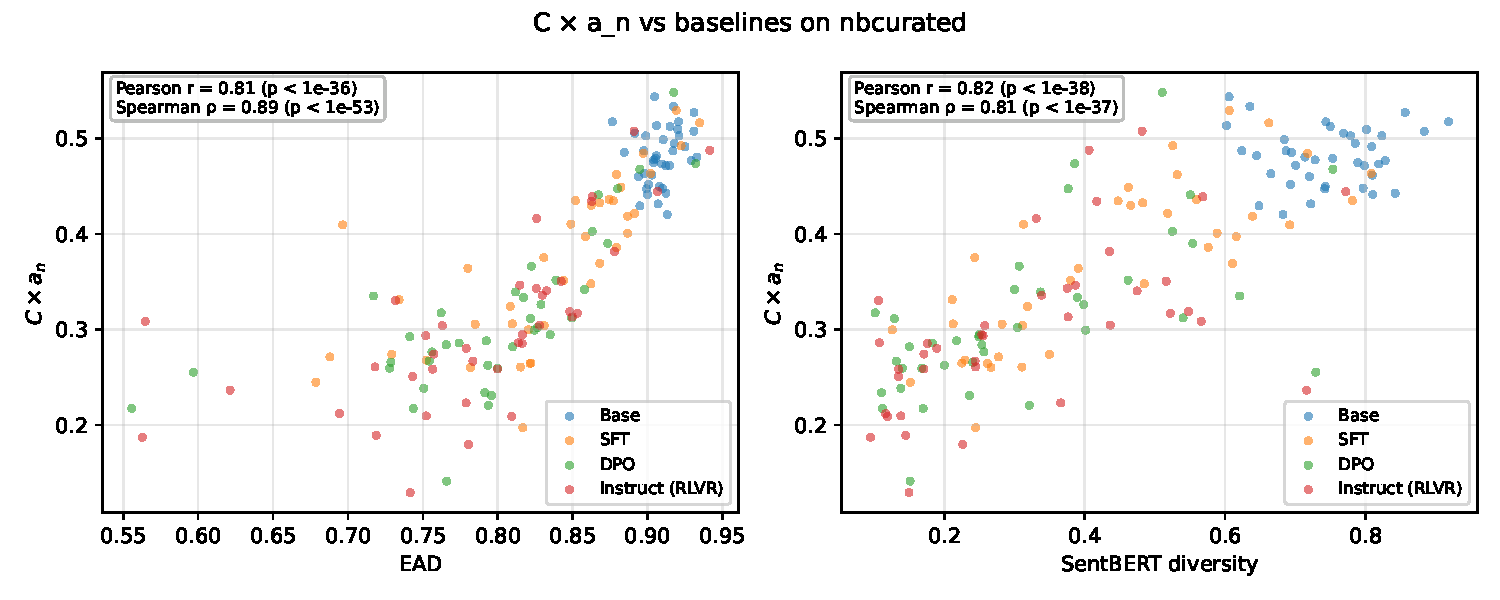
\includegraphics[width=0.85\textwidth]{../figures/rlhf_experiment/metric_correlation_scatter_nbcurated_lm.pdf}
    \caption{NoveltyBench curated (length-matched, $n=\olmoLmNbCuratedN$ prompts).}
\end{subfigure}
\caption{Per-prompt $D_{Ca_n}$ versus EAD (left subpanel) and SentBERT-similarity diversity (right subpanel), coloured by stage, on the length-matched subset of prompts. Length-matching truncates each (stage, prompt) tuple's responses to a common per-prompt byte budget so the per-byte conditional surprise that defines $a_n$ is not depressed by response length. Pearson $r$ and Spearman $\rho$ (two-sided $p$) are reported in each panel. The rank correlations are positive across both prompt sets and both baselines: $D_{Ca_n}$ tracks the same diversity-loss signal EAD and SentBERT detect, and the agreement is not an artefact of response length.}
\label{fig:rlhf-metric-scatter}
\end{figure*}
}{}

\paragraph{Discussion.} The monotone drop across all three pre-registered contrasts is consistent with the post-training-reduces-diversity findings of \citet{kirk2023rlhf,padmakumar2023writingreduces}, now measured by an information-theoretic metric that needs neither an embedding model nor a sentence similarity function.
Cross-metric agreement with EAD and SentBERT (Figure~\ref{fig:rlhf-metric-scatter}) confirms $D_{Ca_n}$ responds to the same signal lexical and semantic baselines detect.
The within-pipeline drop ($\sim$\olmoNbCuratedBaseDMean{} to \olmoNbCuratedInstructDMean{}, about 0.2 bits/byte across the four OLMo stages) is comparable in magnitude to the dispersion observed across an entire frontier instruct-model cluster on the same NoveltyBench-curated prompts; we defer the full cross-model table to a longer venue.

\paragraph{Released artefacts.} The \olmoAlpacaN$\,+\,$\olmoNbCuratedN{} prompts $\times$ 4 stages $\times$ $K{=}10$ generations are released as a public dataset (link withheld for double-blind review; an anonymous mirror is in supplementary materials).
To our knowledge this is the first public release of $K\!\ge\!10$ sampled responses across a paired SFT/DPO/RL pipeline, filling a gap that blocked direct diversity replication of \citet{kirk2023rlhf} (whose $K{=}16$ generations were logged only to a private W\&B project).

% --- macro fallbacks (only fire if the generated files are absent) ---
\providecommand{\olmoAlpacaN}{200}
\providecommand{\olmoNbCuratedN}{100}
\providecommand{\olmoAlpacaBaseDMean}{??}
\providecommand{\olmoAlpacaSftDMean}{??}
\providecommand{\olmoAlpacaDpoDMean}{??}
\providecommand{\olmoAlpacaInstructDMean}{??}
\providecommand{\olmoAlpacaHoneADz}{??}
\providecommand{\olmoAlpacaHoneAPbonf}{??}
\providecommand{\olmoAlpacaHoneBDz}{??}
\providecommand{\olmoAlpacaHoneBPbonf}{??}
\providecommand{\olmoAlpacaHoneCDz}{??}
\providecommand{\olmoAlpacaHoneCPbonf}{??}
\providecommand{\olmoAlpacaHpaDiff}{??}
\providecommand{\olmoAlpacaHpaDz}{??}
\providecommand{\olmoNbCuratedBaseDMean}{??}
\providecommand{\olmoNbCuratedSftDMean}{??}
\providecommand{\olmoNbCuratedDpoDMean}{??}
\providecommand{\olmoNbCuratedInstructDMean}{??}
\providecommand{\olmoNbCuratedHoneADz}{??}
\providecommand{\olmoNbCuratedHoneAPbonf}{??}
\providecommand{\olmoNbCuratedHoneBDz}{??}
\providecommand{\olmoNbCuratedHoneBPbonf}{??}
\providecommand{\olmoNbCuratedHoneCDz}{??}
\providecommand{\olmoNbCuratedHoneCPbonf}{??}

% Length-matched run macros (only the prompt counts are referenced here)
\providecommand{\olmoLmAlpacaN}{??}
\providecommand{\olmoLmNbCuratedN}{??}

% Cross-model comparison table macros
\providecommand{\crossModelOlmoBase}{??}
\providecommand{\crossModelOlmoSft}{??}
\providecommand{\crossModelOlmoDpo}{??}
\providecommand{\crossModelOlmoInstruct}{??}
\providecommand{\crossModelQwenFourB}{??}
\providecommand{\crossModelQwenEightB}{??}
\providecommand{\crossModelQwenTwoThreeFiveB}{??}
\providecommand{\crossModelLlamaThreeThreeSeventyB}{??}
\providecommand{\crossModelGptFiveNano}{??}
\providecommand{\crossModelGptFive}{??}
\providecommand{\crossModelClaudeSonnetFourFive}{??}
